\chapter{Framework Implementation}

In this chapter the description of the framework development is given. It is intended to provide implementation details of a presented concept for a chosen stack of technologies. Based on a workflow of the framework outlined above, separate modules were implemented. Detailed description of each of them is presented in following sections. First sections circumstantiate processing and approximating the input trajectory data. Further sections present the details of the solution implementation to solve tasks of clustering, clusters modeling and input trajectory classification. Since no appropriate ready frameworks providing chosen algorithms were found, all the algorithms implementations, except polynomial regression and polynomial equations solving, were written from scratch and are presented in the Appendix chapter.

\section{Stack of Technologies}

For implementation part of the work Java programming language along with libraries and Apache Maven as a build automation tool were used with following versions:
\begin{itemize}
	\item Java - 11 OpenJDK
	\item Apache Maven - 3.6.3
	\item Commons Math: The Apache Commons Mathematics Library - 3.4.1
	\item Java AWT, Javax Swing 
\end{itemize}

Java was used as a main programming language of an implemented framework. Commons Math library was chosen for approximation step since it provides implementations for $PolynomialFunction$ and $PolynomialSolver$ classes. 

Java AWT (Abstract Window Toolkit) is an API (Application Programming Interface) toolkit for providing a GUI (Graphical User Interface) to a Java application and comes as a part of a Java JDK. In this work Java AWT was used primarily to create objects of $BufferedImage$ with an input image and draw trajectory points on them.

Java Swing as well as Java AWT is a GUI widget toolkit pursuing the same objective of providing a GUI to Java applications and creating window-based applications. However, Swing is more recent and advanced and supports more elaborate set of GUI components than Java AWT. In this work Swing was used to create windows with output images to visualize input trajectories, approximation and clustering results.

\section{Input Data Description (Nature of Data)}

According to the research done by the US Department of Transportation based on data of Fatality Analysis Reporting System (FARS) and National Automotive Sampling System, nearly 40 percents of all the reported in 2008 year crashes were road intersection related \cite{inproceedings:10_cfi}. Consequently, cross-road transport activity analysis is significantly important nowadays in context of safety, and identifying unsafe vehicular trajectories, which violate traffic rules, may be one of the steps towards improving the statistics.

In the presented work video from enforcement cameras is used for training and testing. Test videos are captured using the Intellectual Transportation Systems implemented on four different Kazan crossroads:
\begin{enumerate}
	\item An intersection of Pravo-Bulachnaya and Puschkina streets, $1.txt$ (Figure \ref{fig:is_1}).
	\item An intersection of Nesmelova and Kirovskaya Damba streets, $2.txt$ (Figure \ref{fig:is_2}).
	\item An intersection of Moskovskaya and Galiaskara Kamala streets, $3.txt$ (Figure \ref{fig:is_3}).
	\item An intersection of Moskovskaya and Parizhskoy Kommunyi streets, $4.txt$ (Figure \ref{fig:is_4}).
\end{enumerate}

Each crossroad corresponds to a 4-way intersection and is equipped with a single monitoring camera. Sample pictures from surveillance cameras are given below on Figure \ref{fig:is_all}.

\begin{figure}[!htb]
	\centering
	\begin{subfigure}[!htb]{0.48\textwidth}
		\centering{}
		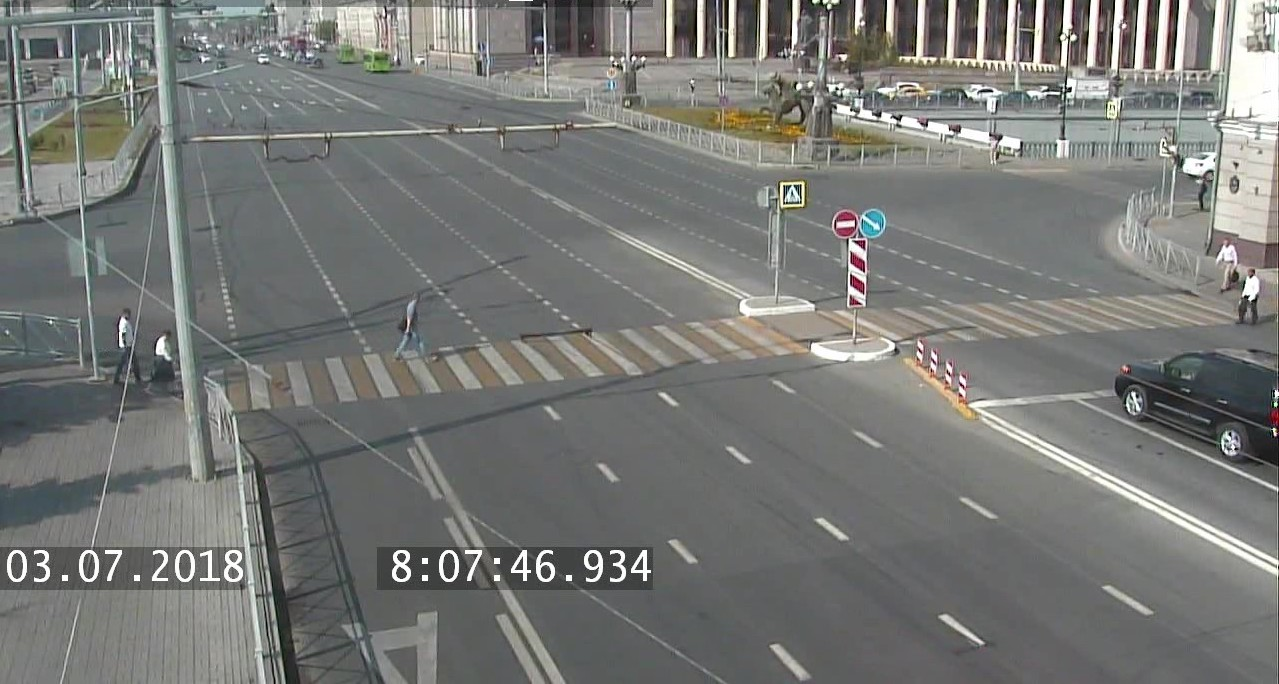
\includegraphics[width=\textwidth]{images/is-1.jpg}
		\caption{$1.txt$}
		\label{fig:is_1}
	\end{subfigure}
	\hfill
	\begin{subfigure}[!htb]{0.48\textwidth}
		\centering{}
		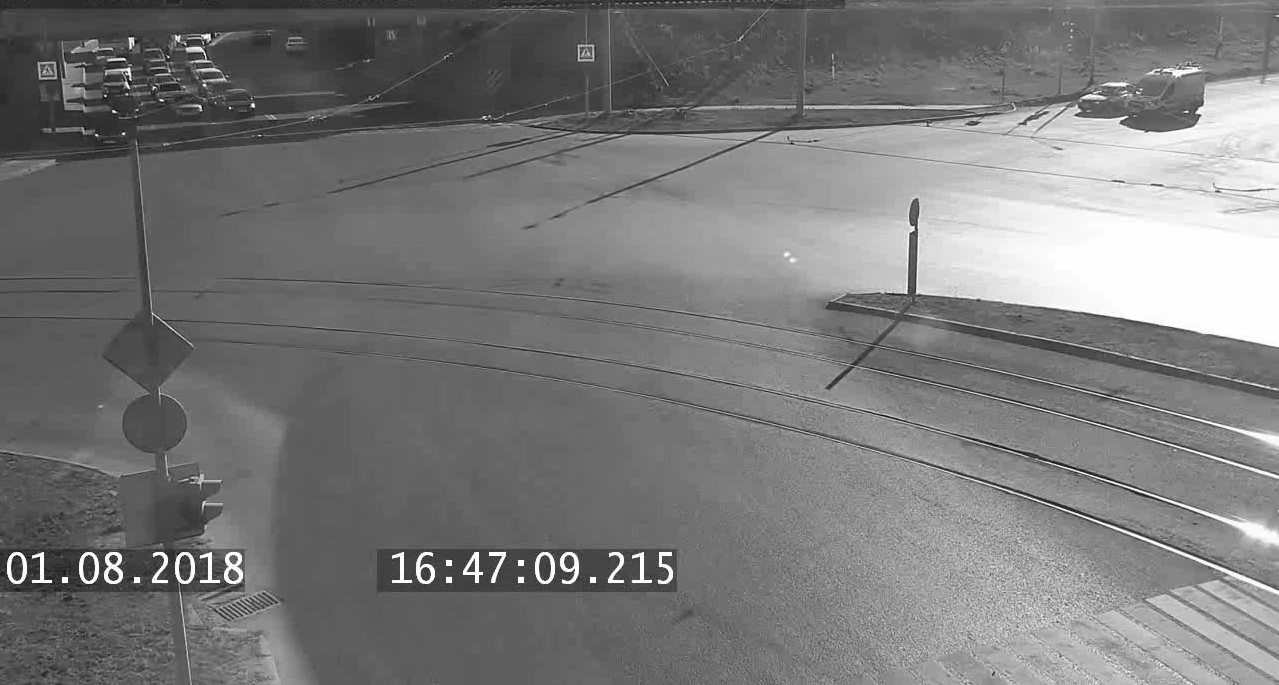
\includegraphics[width=\textwidth]{images/is-2.jpg}
		\caption{$3.txt$}
		\label{fig:is_2}
	\end{subfigure}
	\hfill
	\begin{subfigure}[!htb]{0.48\textwidth}
		\centering{}
		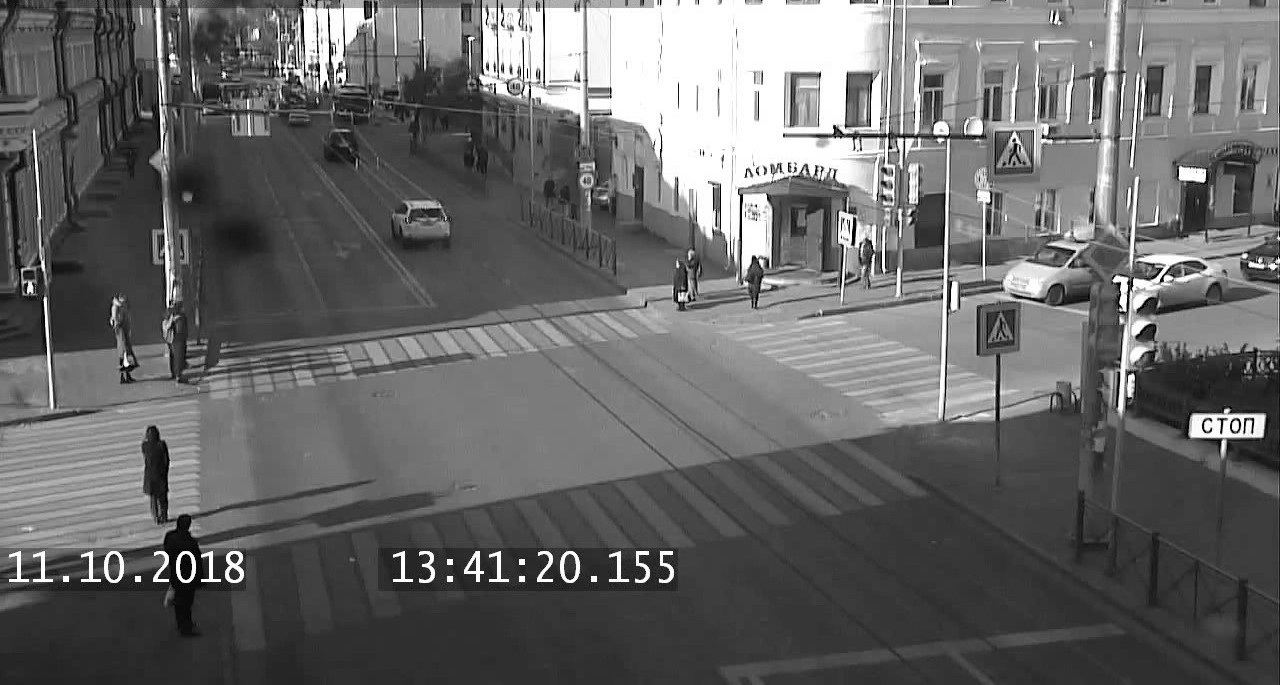
\includegraphics[width=\textwidth]{images/is-3.jpg}
		\caption{$4.txt$}
		\label{fig:is_3}
	\end{subfigure}
	\hfill
	\begin{subfigure}[!htb]{0.48\textwidth}
		\centering{}
		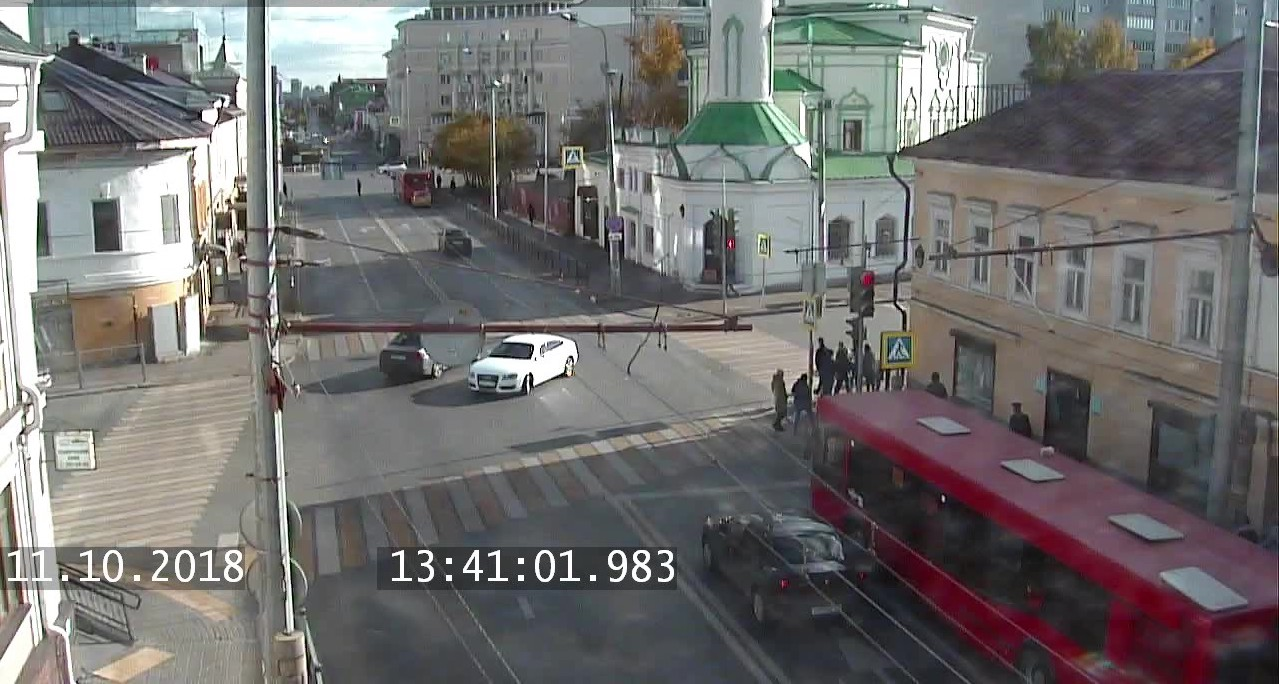
\includegraphics[width=\textwidth]{images/is-4.jpg}
		\caption{$4.txt$}
		\label{fig:is_4}
	\end{subfigure}
	\caption{Input data sources, intersections 1-4}
	\label{fig:is_all}
\end{figure}

Input data files contain 624, 211, 231, 237 vehicular trajectories for the each of the aforementioned intersections respectively.

By a trajectory anomaly we understand vehicle trajectories through the crossroad, which remarkably differ from majority of common, known trajectories. For example, if no turning to the right from the left line is allowed, such a behavior will be unknown and such a trajectory must be considered as an anomaly.

\begin{figure}[!htb]
	\centering{}
	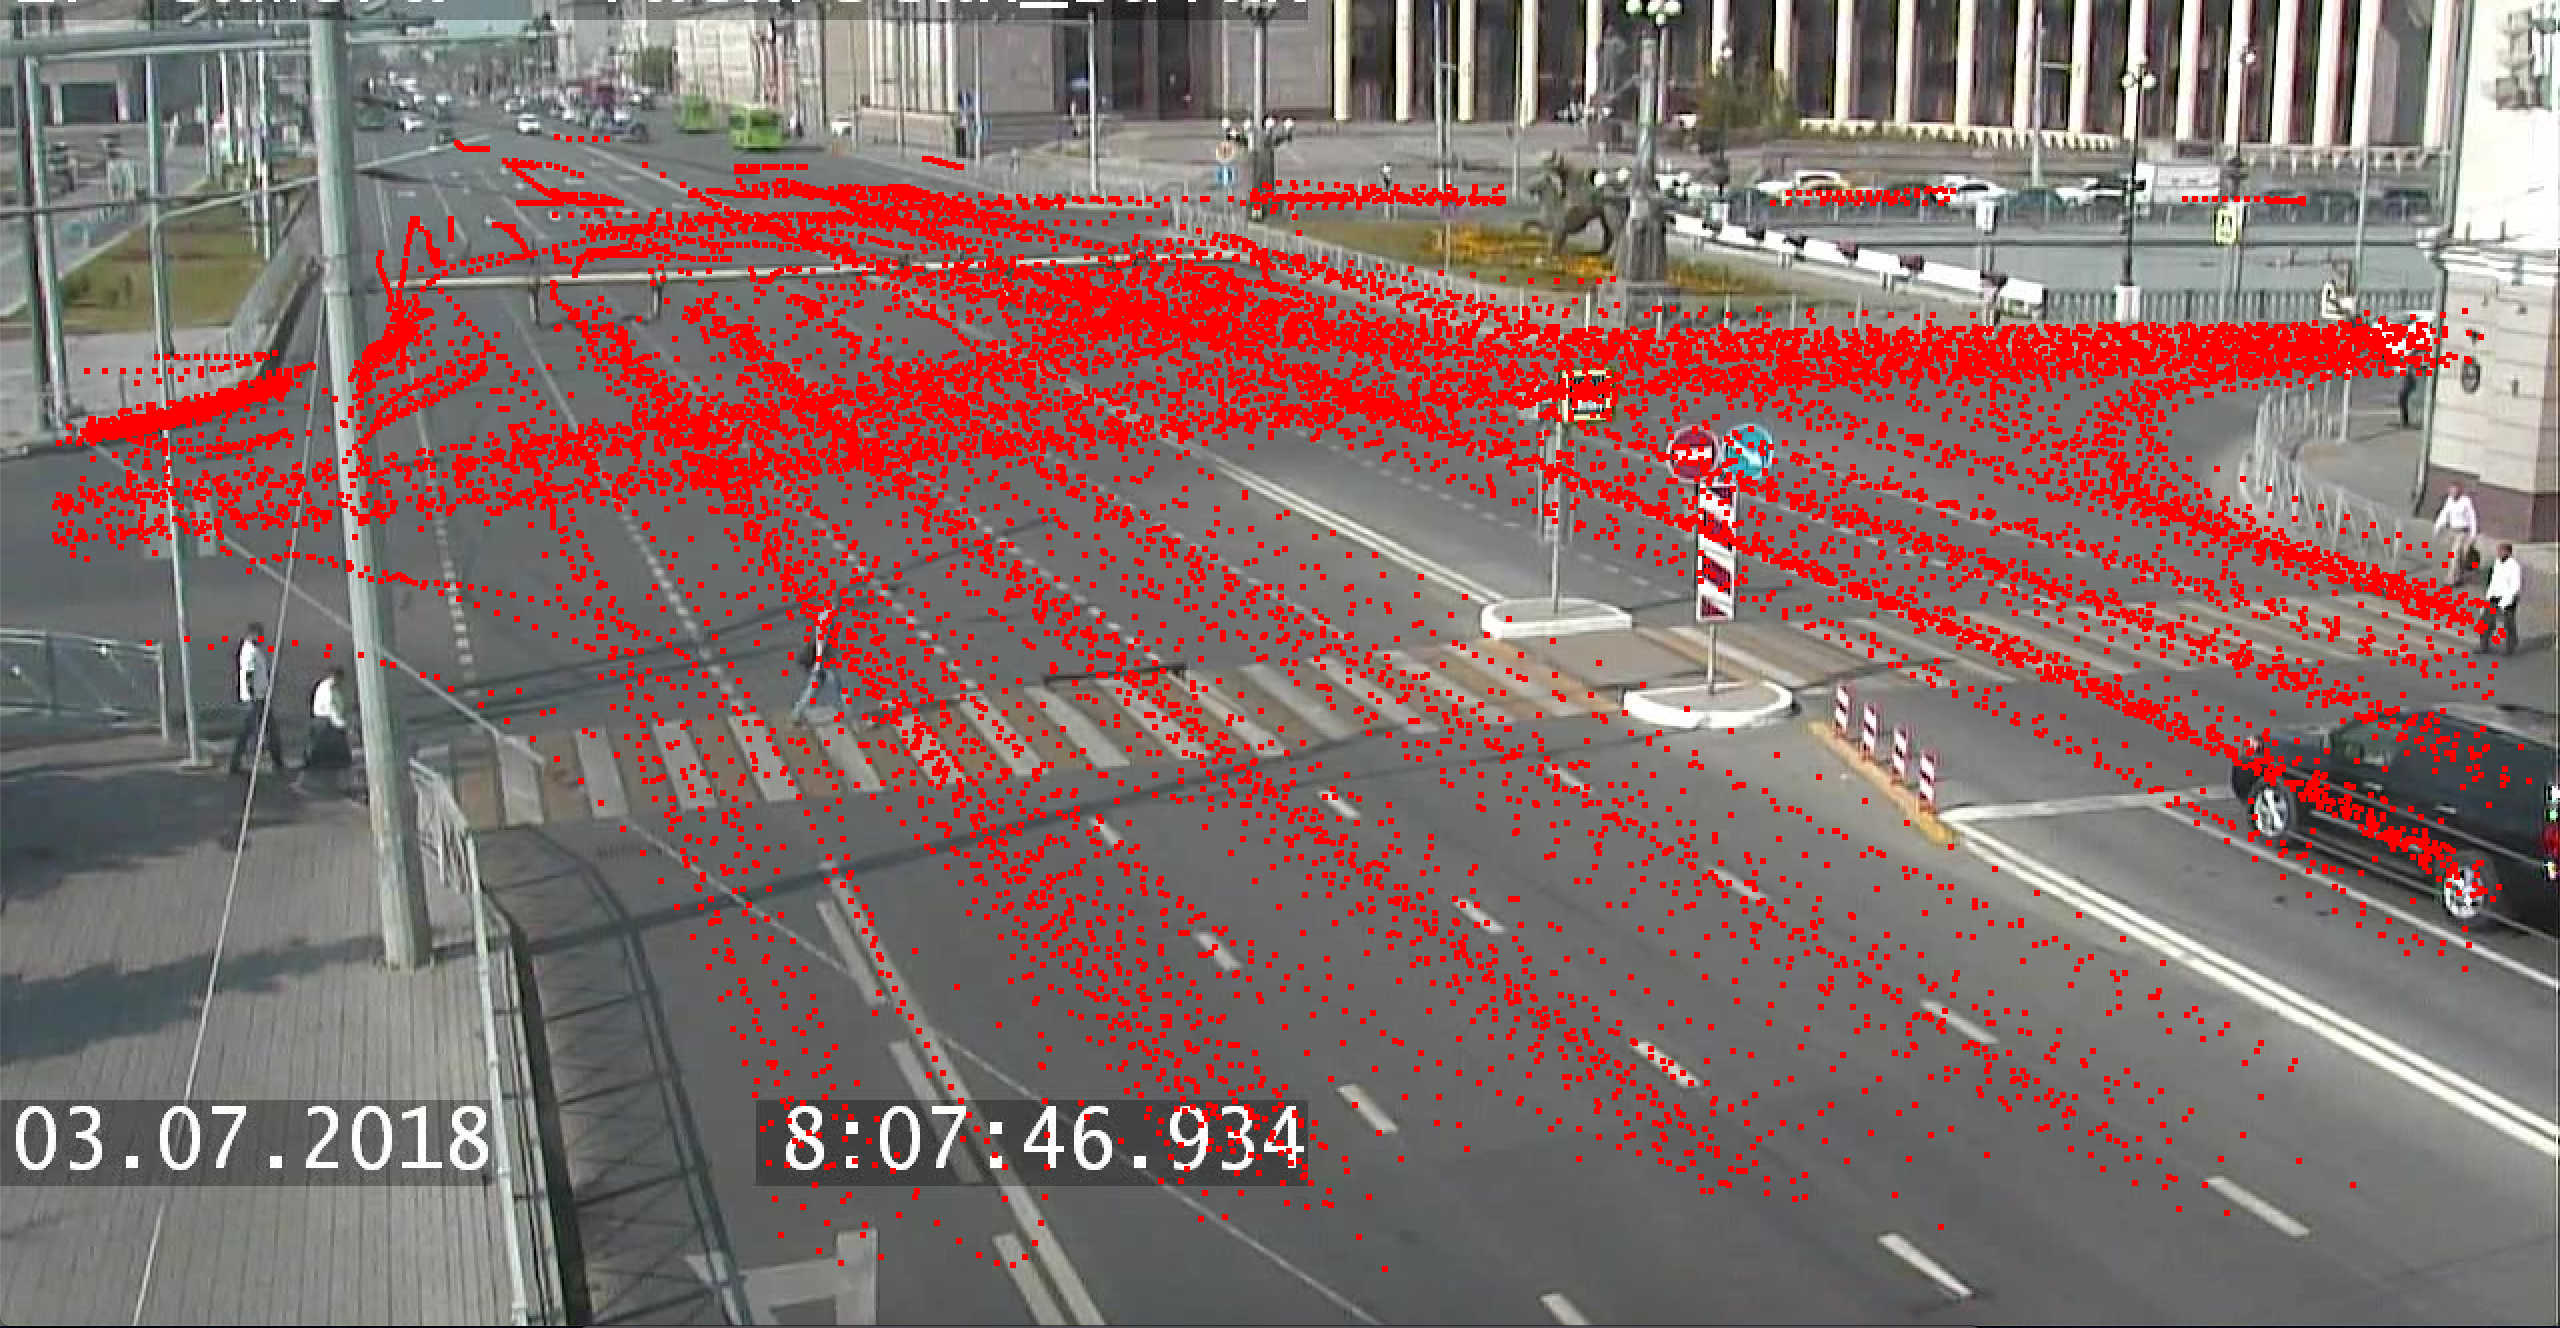
\includegraphics[width=0.8\textwidth]{images/tr-p.png}
	\caption{Output of a tracking system for video the first intersection}
	\label{fig:tr_p}
\end{figure}

\subsection{Input data file structure}
Tracking system, as it was described before, handles video from enforcement cameras and prepare it for further analysis: converts video stream into a set of vectors with tracking points on images (Figure \ref{fig:tr_p}).

Input data files have the following structure:
\begin{equation} \label{eq:input_str}
[[[(x_1^1, y_1^1), ..., (x_1^n, y_1^n)], [t_1, ... t_n]], [[(x_2^1, y_2^1), ..., (x_2^m, y_2^m)], [t_1, ... t_m]], ...]
\end{equation}

As it can be seen from the input data file structure, each trajectory is represented by a two-element array, where first array stores coordinates as an array of two-tuples $(x_i^j, y_i^j)$ and second array contains timestamps for each spatial point in the corresponding order $(t_i)$. The extracted $x$- and $y$-coordinates correspond to pixels on input images. In Formula \ref{eq:input_str} the lower index of the spatial coordinates indicates the ordering number of a trajectory, while the upper index indicates the ordering number of a tracking point. The outer array refers to the array of trajectories.

\section{Input Data Processing}
Since chosen algorithm requires trajectories in a form of multi-dimensional vectors, the initial input data needs to be converted into the required form. For that reason, a custom parser was implemented. It takes a ‘txt’ file with trajectories as an input and as a result it returns a list of Trajectory objects. Trajectory object consists of a number of TrajectoryPoint objects with following information: \textit{x}-coordinate, \textit{y}-coordinate, time \textit{t}. The source code of the parsing method is presented in Appendix A.

Input data contains trajectories of different length and covered distance. However, due to accuracy and tracking errors in tracking system, some trajectories are senseless and look deficient. One of the possible reasons of that is losing the tracking object by a tracker. In contrast with the case of lost location, then the missed location can be found using approximation and regression models, the lost tracking object can not be fixed afterwards. for that reason, in order to improve the quality of results, it was decided to filter the input trajectories and ignore short trajectories with small covered distance, where the covered distance is calculated as an Euclidean distance between first and last trajectory points. For filtering parameters following values were used: $minLength = 10\ (trajectory\ points)$, $minTotalDist = 80\ (pixels)$. Filtering results with depicting the removed and kept trajectories are showed in Figure \ref{fig:traj_filter}.

\begin{figure}
	\centering
	\begin{subfigure}[b]{0.48\textwidth}
		\centering{}
		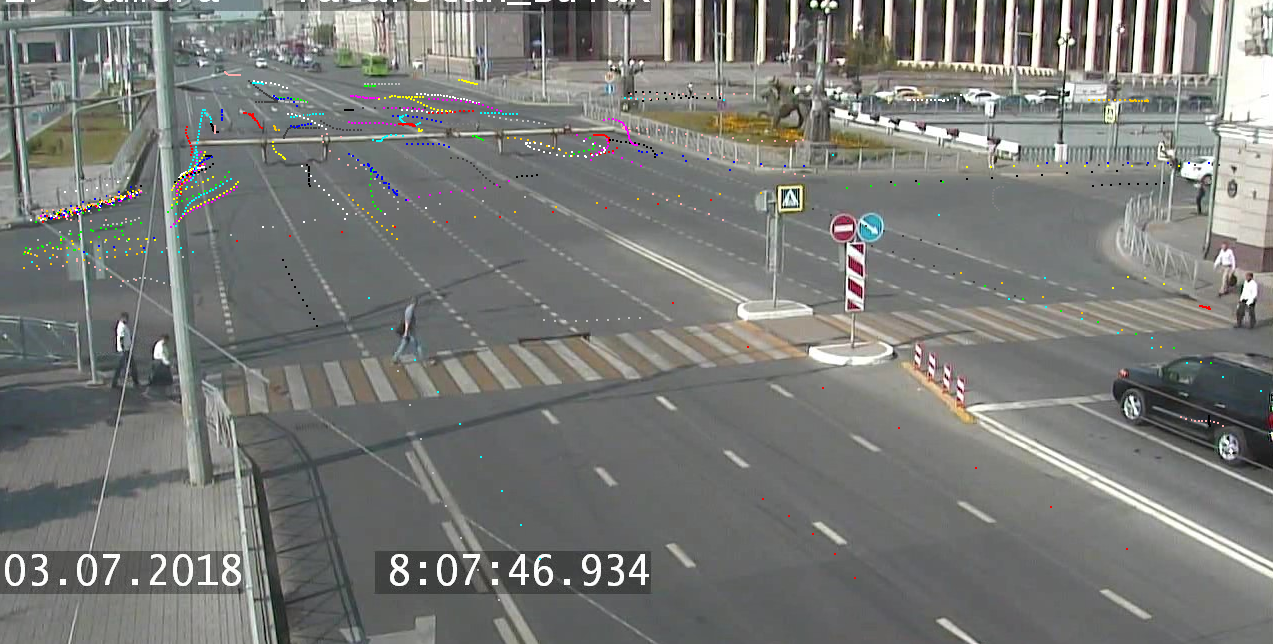
\includegraphics[width=\textwidth]{images/traj-filter-out.png}
		\caption{ignored}
		\label{fig:traj_filter_out}
	\end{subfigure}
	\hfill
	\begin{subfigure}[b]{0.48\textwidth}
		\centering{}
		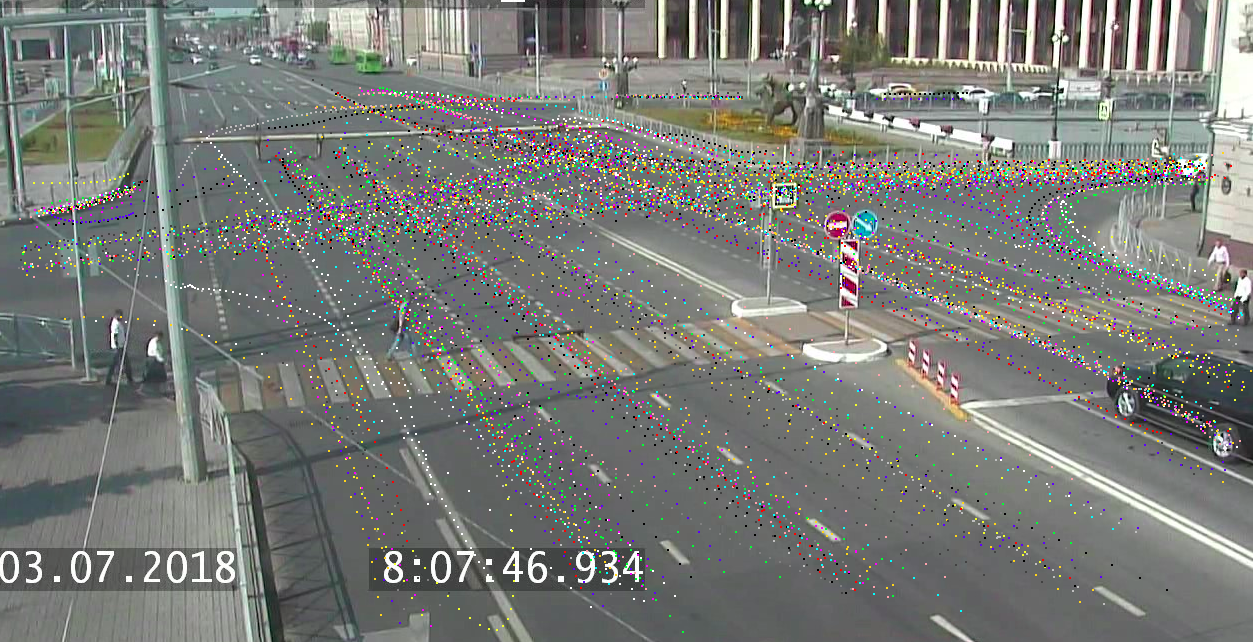
\includegraphics[width=\textwidth]{images/traj-filter-keep.png}
		\caption{$3.txt$}
		\label{fig:traj_filter_keep}
	\end{subfigure}
	\caption{Results of trajectories filtering for $1.txt$}
	\label{fig:traj_filter}
\end{figure}

As it was mentioned before, the current work is focused on detecting two types of abnormalities: spatial and spatiotemporal. To detect the outliers of the first group it is sufficient to analyze spatial information of trajectories. Detecting outliers of the second group, which is formed by trajectories of vehicles moving with an anomalously low or high speed, requires taking into consideration the temporal information along with spatial. For that reason the average constant speed $\upsilon$ is being calculated for each of the input trajectories $t$ at the end of the parsing step using the following equation (Formula \ref{eq:avg_speed}):

\begin{equation} \label{eq:avg_speed}
\upsilon_{avg}(t) = \frac{distance_{total}} {time_{total}},
\end{equation}

where $distance_{total}$ refers to the total distance between the first and last trajectory points and $time_{total}$ refers to the time elapsed. The total distance can be computed as a sum of Euclidean distances between trajectory points on neighboring frames. Since it is known that frames are taken with an inter-frame interval 0,01 second, the speed calculation can be implemented as follows (Listing \ref{lst:speed-calc}):

\lstset{style=code-style-java}
\lstinputlisting[caption={Speed calculation}, label={lst:speed-calc}] {listings/calcSpeed.java}

\section{Trajectories Approximation using Polynomial Regression}

As it was discussed before, the polynomial regression will be used to approximate input trajectories. The implementations of a polynomial entity class\footnote{Polynomial implementation \url{https://javadoc.io/doc/org.apache.commons/commons-math3/3.4.1/org/apache/commons/math3/analysis/polynomials/PolynomialFunction.html}} (needed to further analyze the approximation equations and find key points) and a polynomial equation solver \footnote{Polynomial Function Solver implementation \url{https://www.javadoc.io/doc/org.apache.commons/commons-math3/3.4.1/org/apache/commons/math3/analysis/solvers/LaguerreSolver.html}} from the Apache Commons Math 3.4.1 library were used. To perform a polynomial regression\footnote{Polynomial Regression implementation \url{https://algs4.cs.princeton.edu/14analysis/PolynomialRegression.java}} the implementation provided by R. Sedgewick and K. Wayne for Java language was taken \cite{online:polynomial_impl}. All the ready-to-use implementations were extended by utility methods.

The $PolynomialRegression$ class takes as an input the desired degree of a polynomial ($d$) and two data sets of N data points consisting of real numbers: array of independent variables ($double[] t$), temporal data in this case, and array of dependent variables ($double[] x$, $double[] y$), spatial $x$- or $y$-coordinates. Then it performs a polynomial regression on an input set of N data points $(t_i, x_i)$ or $(t_i, y_i)$ and tries to fit a polynomial $x = \beta_0 + \beta_1t + \beta_2t^2 + \ldots \beta_dt^d$, where $\beta_i$ are the regression coefficients, with an aim to minimize the sum of squared residuals of the multiple regression model. Finding the best solution for polynomial parameters is based on a Least Squares method \cite{article:behav_form_extr}.

In order to achieve better approximation the evaluation of polynomial regression results was performed using the Coefficient of Determination denoted by $R^2$ (also known as a $R$-$squared$ score, \textit{Pearson's coefficient of regression}) \cite{inbook:stats}. $R^2$ measures the proportion of the response dependent variable variance that can be explained by the regression model with given parameters and is predictable from the independent variable and can be calculated as follows: 

\begin{equation}\label{eq:r_sq}
	R^2 = 1 - \frac{SSE}{TSS} = 1 - \frac{\sum{(y_i - \hat{y_i})^2}}{\sum{(y_i - \overline{y})^2}}
\end{equation}

where $SSE$ (Sum of Squares due to Error) is calculated as a sum of squared differences between actual $y_i$, and predicted $\hat{y_i}$ dependent variable values and $TSS$ (Total Sum of Squares) is calculated as a sum of squared deviations of an actual value $y_i$ from a mean $\overline{y}$.

$R^2$ takes a value between [0, 1] and value of 1 indicates that the model (polynomial equation in this case) predicts the data perfectly \cite{online:reg_r_interpr}. 

In this work the polynomial regression was performed for all the input trajectories (Appendix B). The resulting regression models were compared in terms of $R^2$ score and analyzed with respect to a trajectory: shape, speed. The following Evaluation Chapter will give the comparison of evaluation results and discuss the obtained results.

\subsection{Choosing key points from approximated trajectories}

Using the approximated trajectories in further calculation was aimed to decrease the complexity of LCSS calculation. For that reason the length of trajectories must be reduced by choosing several key representative points from the trajectories by analyzing the approximation polynomials.

It is known from Mathematics that critical points of a polynomial $f(t)$ refer to points where the polynomial function is not differentiable or the derivative at that point is equal to zero (stationary points). Stationary points, including local minimum and maximum, rising and falling inflection points, can be found by analyzing the first derivative of a function and solving the $f'(t) = 0$ equation. The inflection points can be found by further analysis of a second derivative: they correspond to the solutions of $f''(t) = 0$ equation. To solve polynomial equations solvers from Apache Commons Math library were used: $LaguerreSolver$, $BisectionSolver$ with following input parameters:
\begin{itemize}
	\item $maxItem = 30000$ -- sets the maximum allowed iterations to find a solution,
	\item $min = firstTimePoint$ -- defines the minimum allowed value for the solution, means the lower border for a solution;
	\item $max = lastTimePoint$ -- defines the maximum allowed value for the solution, means the upper border for a solution;
	\item $startValue = min + 1$ -- specifies from which value the solver will start searching for a real solution.
\end{itemize}

The equation solvers were run for first and second derivative polynomial functions taken from polynomials for $X$- and $Y$-coordinates. The initiation of a solver is given in Listing \ref{lst:solver-init}:

\lstinputlisting[caption={Polynomial Solver initiation}, label={lst:solver-init}] {listings/initSolver.java}

Solutions found by two solvers are merged together: only points referencing to different to time points are being left.
In the case of trajectories analysis inflection points are very significant, because they carry an important information about the shape of a trajectory: such key points can denote the main turns or changes in the trajectory.

However, critical points can not be always found due to computational restrictions of high-order polynomial functions. Consequently, critical points, identified in such a way, can not fully describe the input trajectory and are not sufficient for further analysis since do not provide all the information about borders of a trajectory shape and sometimes can not visualize all the turns. For that reason it was decided to add key points calculated as border points for a trajectory by taking separately minimum and maximum $X$ and $Y$ coordinates and computing the corresponding trajectory points using a respective regression model (Listing \ref{lst:key-borders-calc}).

\lstinputlisting[caption={Calculating the border coordinates and corresponding key points}, label={lst:key-borders-calc}] {listings/calcKeyBorders.java}

The results of performed polynomial regression approximation and key points calculation are presented in Figure \ref{fig:regr-kp}. The original trajectory data is visualized using a red color, while the blue trajectory points correspond to data points obtained using the functions of a polynomial approximation for the same time points. Key points of each trajectory are emphasized using bold blue square dots. It can be seen that the approximation function is close to the original trajectory function, for some trajectories approximation gives the same coordinates as in the original data (for trajectories with approximation polynomials having $R^2 \approx 1.0$). Also key points accurately follow the approximation line and describe the trajectory properly, hence, they can be used instead of original trajectory points to simplify the further trajectories analysis. 

\begin{figure}[!htb]
	\centering
	\begin{subfigure}[!htb]{0.68\textwidth}
		\centering{}
		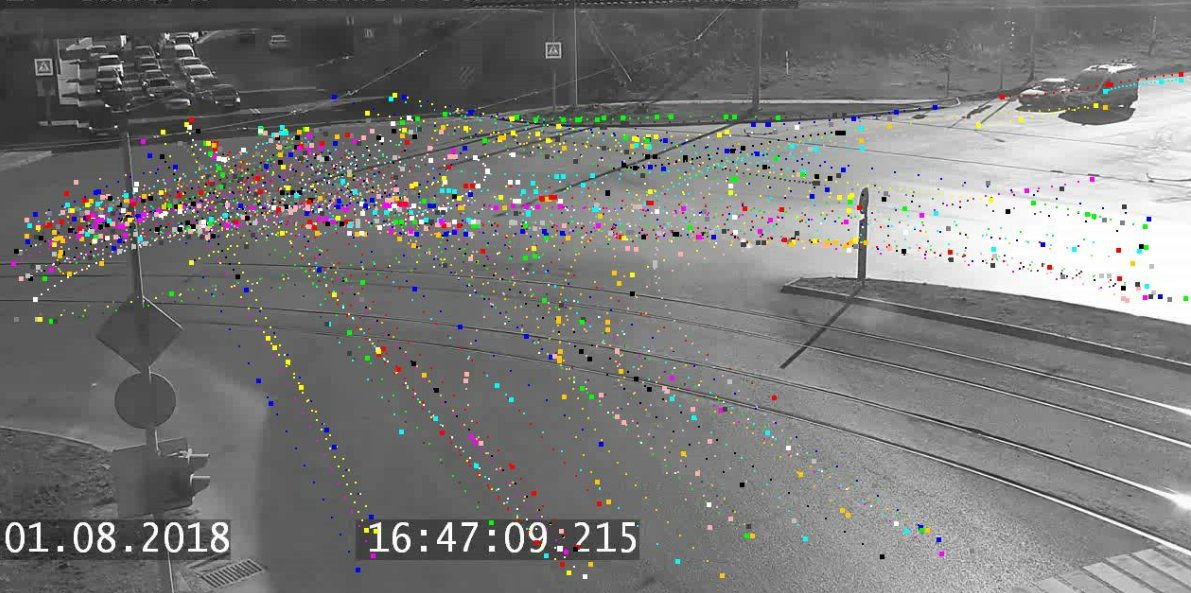
\includegraphics[width=\textwidth]{images/regr_kp_full.png}
		\caption{full $2.txt$}
	\end{subfigure}
	\hfill
	\begin{subfigure}[!htb]{0.3\textwidth}
		\centering{}
		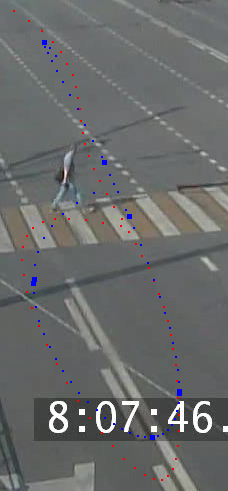
\includegraphics[width=\textwidth]{images/regr_kp_loop.png}
		\caption{loop from $1.txt$}
	\end{subfigure}
	\hfill
	\begin{subfigure}[!htb]{0.3\textwidth}
		\centering{}
		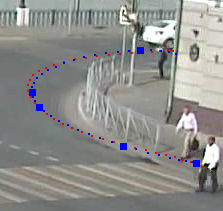
\includegraphics[width=\textwidth]{images/regr_kp_turn.png}
		\caption{turn from $1.txt$}
	\end{subfigure}
	\hfill
	\begin{subfigure}[!htb]{0.3\textwidth}
		\centering{}
		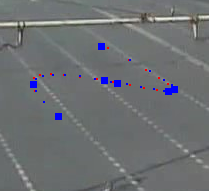
\includegraphics[width=\textwidth]{images/regr_kp_complex.png}
		\caption{complex $1.txt$}
	\end{subfigure}
	\hfill
	\begin{subfigure}[!htb]{0.3\textwidth}
		\centering{}
		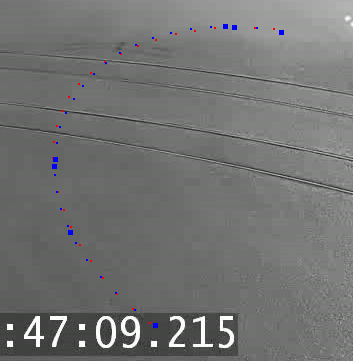
\includegraphics[width=\textwidth]{images/regr_kp_curve_2.png}
		\caption{curve from $2.txt$}
	\end{subfigure}
	\hfill
	\begin{subfigure}[!htb]{0.3\textwidth}
		\centering{}
		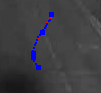
\includegraphics[width=\textwidth]{images/regr_kp_complex_3.png}
		\caption{complex from $3.txt$}
	\end{subfigure}
	\hfill
	\begin{subfigure}[!htb]{0.3\textwidth}
		\centering{}
		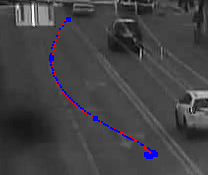
\includegraphics[width=\textwidth]{images/regr_kp_curve_3.png}
		\caption{curve from $3.txt$}
	\end{subfigure}
	\hfill
	\begin{subfigure}[!htb]{0.3\textwidth}
		\centering{}
		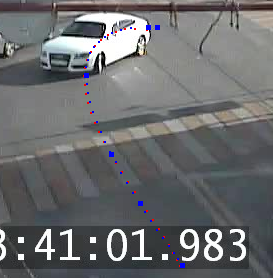
\includegraphics[width=\textwidth]{images/regr_kp_curve_4.png}
		\caption{curve from $4.txt$}
	\end{subfigure}

	\caption{Results of polynomial regression with emphasizing key points}
	\label{fig:regr-kp}
\end{figure}

\section{Similarity measure calculation}

As it was mentioned before, LCSS measure will be used as a similarity measure. Consequently, LCSS distance will be calculated based on a LCSS similarity according to above mentioned formulas. It is worth noting that LCSS distance is symmetric and for pair of trajectories can be computed just once \cite{inproceedings:28_lcss_dsmt}.

Notwithstanding that the implementation of LCSS similarity measure exists in R package \cite{online:r_lcss}, it does not allow $\delta$ and $\varepsilon$ parameters to be dynamic. For that reason the custom implementation was written. The method for LCSS calculation is presented in Listing \ref{lst:lcss-calc}. 

\lstinputlisting[caption={LCSS calculation}, label={lst:lcss-calc}] {listings/calcLCSS.java}

\section{Clustering}

Since no appropriate implementation of hierarchical clustering for trajectories with the use of LCSS distance and capable of taking an adaptable parameters values were found, the clustering as well as LCSS similarity calculation was written from scratch guided by Algorithm \ref{algo:ahc-descr} outlined above. The source code of clustering is given in Appendix C. 

Clustering is done in an iterative way of joining two closest clusters into one with following recalculation of a clusters similarity (proximity) matrix. The clustering method takes as an input the $OUTPUT\_CLUSTERS\_COUNT$ parameter which controls when the clustering will stop. If no value is passed, it will be considered as 1 and the clustering will be done till all clusters are merged into one in concordance with the basic algorithm of agglomerative hierarchical clustering.


\subsection{Clusters' modeling}

Clusters modeling implementation